\documentclass[12pt]{article}
\usepackage[letterpaper,margin=1in]{geometry}
\usepackage{amsmath,amsfonts,amssymb}
\usepackage{setspace}
\usepackage{fancyhdr}
\usepackage{lastpage}
\usepackage{chngpage}
\usepackage{graphicx}
\usepackage[protrusion=true,expansion,kerning]{microtype}
\usepackage{url}

% adjust margins:
\topmargin=-0.25in
\evensidemargin=0in
\oddsidemargin=0in
\textwidth=6.5in
\textheight=8.5in
\headsep=0.25in

% document-specific information
\newcommand{\docTitle}{Assignment \#4}
\newcommand{\docSubTitle}{}
\newcommand{\docDate}{}
\newcommand{\docClass}{CS650}
\newcommand{\docInstructor}{Learned-Miller}
\newcommand{\authorName}{Emma Strubell}

% header and footer
\pagestyle{fancy}
\lhead{\authorName}
\chead{\bf\docTitle}
\rhead{\docClass\ -- \docInstructor}   
\lfoot{}
\cfoot{}
\rfoot{\emph{Page\ \thepage\ of\ \pageref{LastPage}}}                          
\renewcommand\headrulewidth{0.4pt}
\renewcommand\footrulewidth{0.4pt}

\begin{document}
I experimented with bin sizes of 16, 32, 64, and 128. The following are my resulting images, all of which are examples aligned computed with a bin size of 64, with the exception of the tree image which was computed with a bin size of 128:

\begin{center}
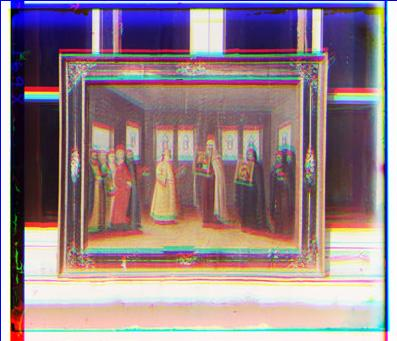
\includegraphics[scale=0.6]{processed/processed-64-00149v.jpg}~
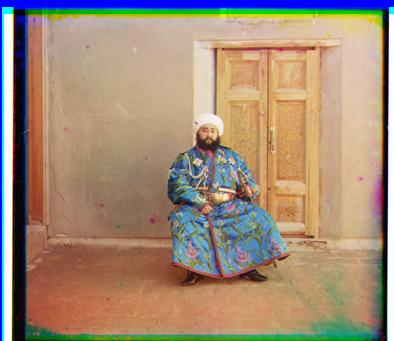
\includegraphics[scale=0.6]{processed/processed-64-00153v.jpg}
\end{center}

\begin{center}
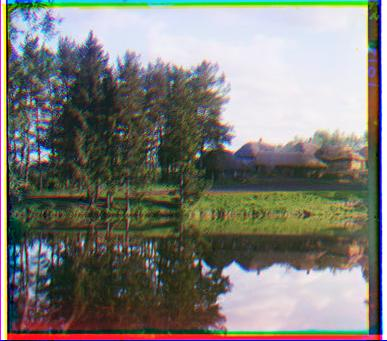
\includegraphics[scale=0.6]{processed/processed-64-00163v.jpg}~
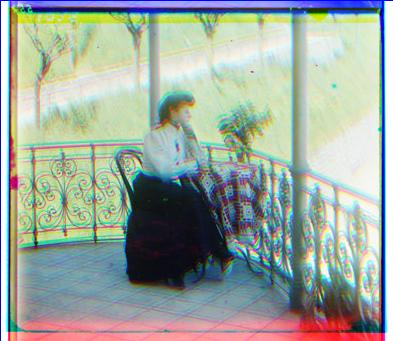
\includegraphics[scale=0.6]{processed/processed-64-00194v.jpg}
\end{center}

\begin{center}
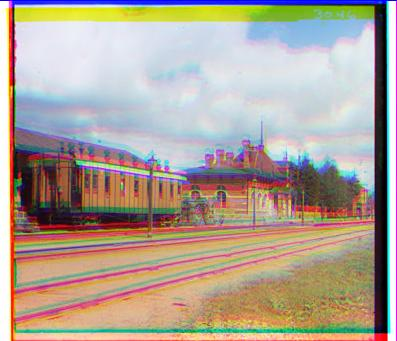
\includegraphics[scale=0.6]{processed/processed-128-00398v.jpg}~
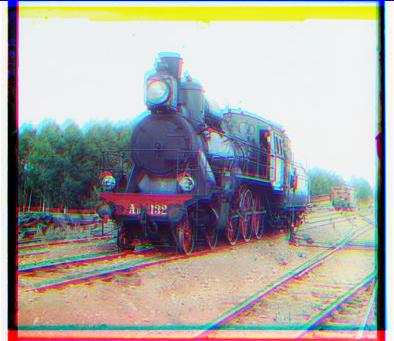
\includegraphics[scale=0.6]{processed/processed-64-00458v.jpg}
\end{center}

\begin{center}
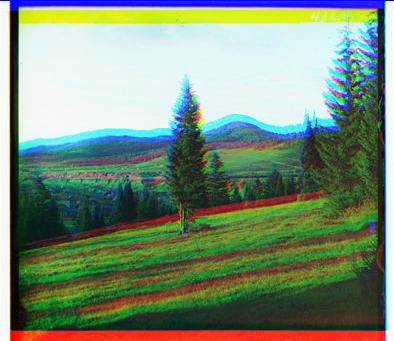
\includegraphics[scale=0.6]{processed/processed-128-00600v.jpg}~
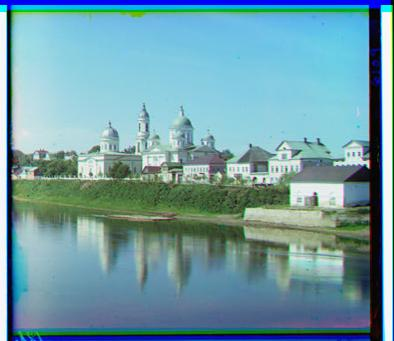
\includegraphics[scale=0.6]{processed/processed-64-01167v.jpg}
\end{center}

I found that the method worked well on most of the images, most of them looking just as aligned using 16 bins as with 128, with the exception of the single-tree image. This means that the coarse histogram often provided enough information about the image to align it without requiring futher binning, which makes sense since we were only shifting the image by 15 pixels anyway.

When I shifted the image, I padded with zeroes, which is the cause for the colorful edges -- a shifted layer with some white padding will allow other colors to show through.

\begin{center}
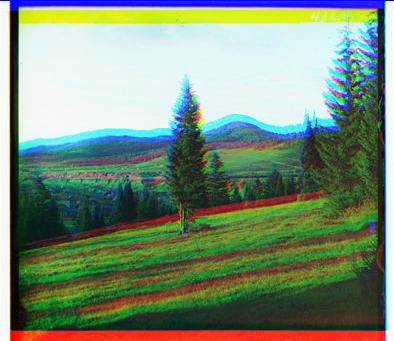
\includegraphics[scale=0.6]{processed/processed-64-00600v.jpg}
\end{center}

The tree image was harder to align compared to the others, requiring more fine-grained binning. Above is the tree image computed using a bin size of 64, which was completely adequate for all the other images. It is clearly poorly aligned. I suspect this has to do with the quality of the image that I aligned to. For all of the images, I just aligned with the first image in the set, the red layer. In most cases, this was fine. In the case of this tree, the red layer is not very informative -- it's mostly used to make the dark parts of the image. So the problem here was likely aligning to a bad image to begin with. If I had aligned to one of the other channels, I expect I would have been able to align this image using a coarser histogram, as with the other images.
\end{document}